% Modelo de relatório no estilo artigo em duas colunas
\documentclass[twocolumn]{article}
\usepackage[utf8]{inputenc}
\usepackage{amsmath}
\usepackage{subcaption}
\usepackage{mathtools}
\usepackage{graphicx}
\usepackage{color}
\usepackage{authblk}
\usepackage{lmodern}
% \usepackage[colorlinks,citecolor=black,urlcolor=black,bookmarks=false,hypertexnames=true]{hyperref}
\usepackage[margin=0.9in]{geometry}
\usepackage{pdfpages}
\usepackage{fancyhdr}
\usepackage[utf8]{inputenc}

\usepackage[sorting=none,style=numeric]{biblatex}
\addbibresource{refs.bib}
\usepackage[justification=centering]{caption}
\usepackage{makecell}
\usepackage{booktabs}
\usepackage{hhline}
\usepackage{amsmath}
\usepackage{amssymb}
\usepackage{soul}
\usepackage{gensymb}
\usepackage{listings}

\setlength\parindent{0pt}


\newcommand{\myname}{Nishant Aswani}
\newcommand{\mynetid}{nsa325}
\newcommand{\myemail}{nsa325@nyu.edu}
\newcommand{\myhwtype}{Lab }
\newcommand{\myhwnum}{7}
\newcommand{\mycoursenumber}{ENGR-UH 3511}
\newcommand{\myclassname}{Computer Organization and Architecture}
\newcommand{\myassignmenttitle}{Microprocessor Design and Verilog HDL: Part 5}
\newcommand{\myinstructor}{Cristoforos Vasilatos}

\newcommand{\cc}[1]{\texttt{#1}}

\lstset{
  basicstyle=\ttfamily,
  escapeinside=||
}

% Tamanho das margens:
% \geometry{
% 	a4paper,
% 	total={170mm,257mm},
% 	left=30mm,
% 	top=20mm,
% }
%%%%%%%%%%%%%%%%%%%%%%%%%%%%%%%%%%%%%%%%%
% Bibliografia estilo ABNT. Se não tiver instalado, comente a linha abaixo.
% \usepackage[alf, abnt-etal-list=0, abnt-emphasize=bf,abnt-last-names=bibtex, abnt-etal-text=it, abnt-etal-cite=2]{abntex2cite}
%%%%%%%%%%%%%%%%%%%%%%%%%%%%%%%%%%%%%%%%%

% Dados de identificação
\title{\myassignmenttitle}
\author{\myname, \myemail}
\affil{\myclassname (\mycoursenumber), Instructor \myinstructor}
\date{}

\begin{document}
%%%%%%%%%%%%%%%%%%%%%%%%%%%%%%%%%%%%%%%%%%%%%%%% COVER PAGE %%%%%%%%%%%%%%%%%%%%%%%%%%%%%%%%%%%%%%%%%%%%%%%%%%%%
\onecolumn
\pagestyle{fancy}
\fancyhf{}
\renewcommand{\headrulewidth}{0pt}
\rhead{\textbf{Division of Engineering}}
\lhead{\textbf{NYU Abu Dhabi}}

\begin{center}
  
\includegraphics[scale=0.15]{etc/NYUAD-alt-logo.jpg}
\end{center}

{\vspace{2.5em}}

\begin{center}
    \Huge{\textbf{\mycoursenumber}}\\
    {\vspace{0.5em}}
    \Huge{\textbf{\myclassname}}
\end{center}

{\vspace{10em}}

\begin{center}
  \begin{tabular}{|rp{5.0cm}lll|}
    \hline
    &  &  &  & \\
    &  &  &  & \\
    \Large{\textbf{Name:}} & \Large{\myname}
    
    \  &  &  & \\
    \Large{\textbf{Net ID:}} & \Large{\mynetid}
    
    \  &  &  & \\
    \Large{\textbf{Assignment Title:}} & \Large{\myhwtype \myhwnum}
    
    \
    
    \  &  &  & \\
    \hline
  \end{tabular}
\end{center}

\

{\newpage}
%%%%%%%%%%%%%%%%%%%%%%%%%%%%%%%%%%%%%%%%%%%%%%%% COVER PAGE %%%%%%%%%%%%%%%%%%%%%%%%%%%%%%%%%%%%%%%%%%%%%%%%%%%%

\maketitle        

% Resumo de no máximo 200 palavras
% \begin{abstract}
% Este documento orienta a descrição das atividades práticas desenvolvidas em laboratório. São usados como exemplo conceitos da Aula 01 de Acionamentos Elétricos sobre partida direta de motor de indução trifásico. Nesta atividade, um motor é acionado com conexões estrela e triângulo a vazio. As correntes nominais e de partida são medidas com amperímetro analógico e comparadas entre si. Nota-se que, mesmo sem carga, as corrente em estrela são maiores. 
% \end{abstract}

\section{Introduction}

Pipelining a CPU improves the instructions throughput in a CPU. However, it may introduce erroneous behavior as certain structures may be simultaneously used at different stages in the pipeline.\\

The following lab uses Verilog to continue an implementation of a 32-bit MIPS CPU. In this lab, two cases of hazards are solved using stalling and two cases are solved using forwarding.
\section{Methodology}

\subsection{Hazard Detection and Stalling}

Two cases of hazard detection and stalling were formulated: Read After Write (RAW) and Load-Use Data Hazard.\\

RAW Hazard
\begin{lstlisting}
    mem[0] <= 32'h21080001;   // addi $t0 $t0 1
    mem[1] <= 32'h21090001;   // addi $t1 $t0 1
\end{lstlisting}
\medskip
Load-Use Data Hazard:
\begin{lstlisting}
    mem[0] <= 32'h8D090000;   // lw   $t1 0(t0)
    mem[1] <= 32'h21290001;   // addi $t1 $t1 2
\end{lstlisting}
\medskip
The pipeline for both programs was drawn out to determine the number of stalls it would require to resolve the issue. The challenge was to select signals from the control, which would keep the stall signal on for long enough for the case to resolve. Looking at the diagrams below, it was discovered that both types required two stalls in the pipeline: 

\newpage 

\begingroup
    \centering
    \medskip
    %width=\columnwidth
    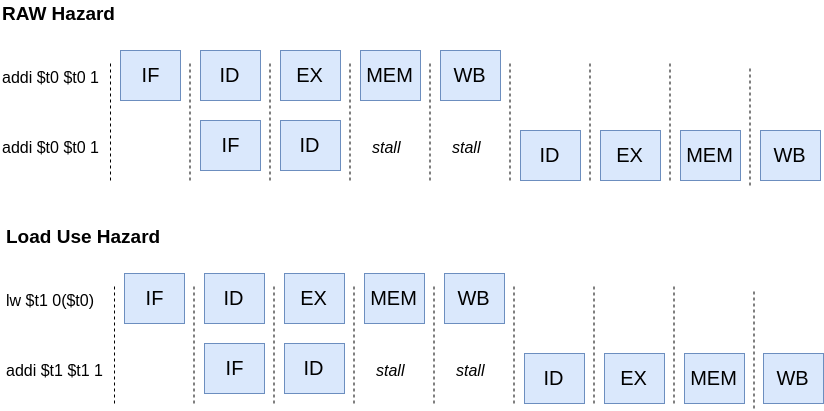
\includegraphics[width=\columnwidth]{Lab-Tex/Lab7-images/stalling_hazard.png}
    \captionof{figure}{Showing the stalls required for both hazard types without forwarding}
    \label{fig:stalling_hazard}
    \medskip
\endgroup

A hazard unit was built to detect both hazard types\\

For the load-use hazard:

\begin{lstlisting}[escapechar=@]
    if (MemRead_ID_EX == 1'b1 && (RegisterRt_ID_EX == RegisterRs_IF_ID @||@
        RegisterRt_ID_EX == RegisterRt_IF_ID)) begin
        Stall_Data_Hazard <= 1'b1;
    end
\end{lstlisting}
\\

The idea is to check if data is being loaded from memory (check MemRead) and if the register it is being loaded to is used again in the next instruction. Looking at Figure \ref{fig:stalling_hazard}, the check is done with these signals because the stall must occur after stage 3 of the first instruction.\\

For the RAW hazard:

\begin{lstlisting}[escapechar=@]
    else if (RegWrite_EX_MEM == 1'b1 && (RegisterRt_ID_EX != 0) &&
            (RegisterRt_ID_EX == RegisterRs_IF_ID ||
            RegisterRt_ID_EX == RegisterRt_IF_ID)) begin

        Stall_Data_Hazard <= 1'b1;

    end
\end{lstlisting}
\\

Here the idea is to check if a register is being written to and if the register it is written to is equal to a register being read in the next instruction. Once again, we use the ID-EX and IF-ID registers for the same reason as above. We use the EX-MEM val for RegWrite because it allows for delaying the stall at the right time, otherwise the stall occurs too early. \\

In the top-level module, the stall signal was fed as the hold signal into the components in stage 1 and stage 2. All the control signals had to be propagated so the stall could end. Otherwise stall would continue on indefinitely. The components in stage 3,4,5 were not fed the stall signal, so the values could be calculated and update the register values appropriately. Although, a new condition was added to the control unit: all control values are set to zero when the stall signal is enabled. This idles the pipeline for the duration of the stall. 
  
\subsection{Hazard Detection and Forwarding}

The first RAW sample program was revisited, this time solved using forwarding. The two forwarding types (EX hazard and MEM hazard) were combined into one program. \\

\begin{lstlisting}
    mem[0] <= 32'h21080001;   // addi $t0 $t0 0x1
    mem[1] <= 32'h21090001;   // addi $t1 $t0 0x1
    mem[2] <= 32'h210A0001;   // addi $t2 $t0 0x1
\end{lstlisting}
\\

A forwarding unit was added to the top-level module and the previous hazard detection unit was left unused. Figure \ref{fig:forwarding} shows the higher level overview of what the forwarding unit does for the program above. \\

\begingroup
    \centering
    \medskip
    %width=\columnwidth
    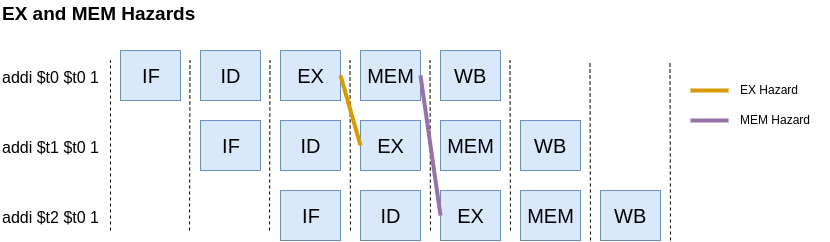
\includegraphics[width=\columnwidth]{Lab-Tex/Lab7-images/forwarding.png}
    \captionof{figure}{How forwarding solves EX and MEM hazards}
    \label{fig:forwarding}
    \medskip
\endgroup

For the EX hazard: 

\begin{lstlisting}[escapechar=@]
    if (RegWrite_EX_MEM == 1'b1 && (RFWriteReg_EX_MEM != 0) &&
            (RFWriteReg_EX_MEM == RegisterRs_ID_EX)) begin

      ForwardA <= 2'b10;
      ForwardB <= 2'b00;
    end

    else if (RegWrite_EX_MEM == 1'b1 && (RFWriteReg_EX_MEM != 0) &&
            (RFWriteReg_EX_MEM == RegisterRt_ID_EX)) begin

      ForwardA <= 2'b00;
      ForwardB <= 2'b10;
    end
\end{lstlisting}
\medskip

The logic above checks if the register write signal is enabled in the 4th stage, if the register being written to (Rd) is not \cc{\$zero}, and if Rd coincides with a register being used in the next instruction. Depending on which register (Rs or Rt) Rd coincides with, the ALU result from the current instruction is forwarded to an input of the ALU for the next instruction. When the Forward signals are \cc{2'b00}, they simply take in the value the register file gives, as if there is no forwarding; it is the default. \\

\newpage

For the MEM hazard:

\begin{lstlisting}[escapechar=@]
    else if (RegWrite_MEM_WB == 1'b1 && (RFWriteReg_MEM_WB != 0) &&
            (RFWriteReg_MEM_WB == RegisterRs_ID_EX)) begin

      ForwardA <= 2'b01;
      ForwardB <= 2'b00;
    end

    else if (RegWrite_MEM_WB == 1'b1 && (RFWriteReg_MEM_WB != 0) &&
            (RFWriteReg_MEM_WB == RegisterRt_ID_EX)) begin

      ForwardA <= 2'b00;
      ForwardB <= 2'b01;
    end
\end{lstlisting}
\medskip

The condition checking here is slightly more rigorous; although, the conditions are very similar. The forwarding unit checks if the register write signal is enabled in the 5th stage, if the Rd in the 5th stage is not zero, and is equal to the Rs or Rt in the 3rd stages. It is imperative that this check occurs after the one for EX hazard. This ensures that when something from the block above is executed, none of the conditions for the EX hazard were met. This is to prevent data hazards when three consecutive instructions all use the same register as their destination register. \\

\section{Results}


\subsection{Hazard Detection and Stalling}

Given the RAW hazard, the pipeline requires two stalls after the first instruction, so that the data can be written back to the register before the next instruction uses that register. \\

Figure \ref{fig:raw_stall} shows that the \cc{PCnext} stalls for two cycles (4th and 5th cycle). Once the value is written back in the 5th cycle, we see that the \cc{PCnext} progresses on the 6th cycle. The two-cycle stall occurs because the \cc{RegWrite-EX-MEM} signal activates and the register comparisons return true. It is also worth noticing that the RegWrite control signal goes to zero, despite the instruction still technically being the \cc{addi} instruction; this is because control is set to zero on all stalls. We see that register \cc{\$t1} receives its value three cycles after \cc{\$t0}, propgating the effect of the two stalls. \\ 

\begingroup
    \centering
    \medskip
    %width=\columnwidth
    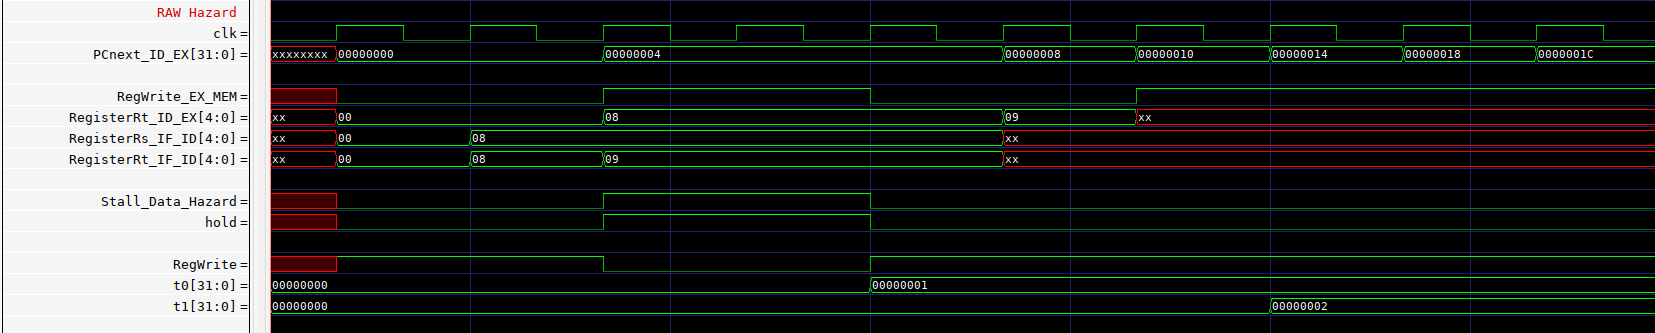
\includegraphics[width=\columnwidth]{Lab-Tex/Lab7-images/p3.png}
    \captionof{figure}{Signals for the RAW hazard in stalling}
    \label{fig:raw_stall}
    \medskip
\endgroup

Given the load use hazard, the pipeline also requires two stalls after the first instruction. In figure \ref{fig:loaduse_stall}, we see that the pipeline once agains stalls at the 4th and 5th cycle. Interestingly, the second stall occurs as a result of the condition being met for the RAW hazard. The control signal for the load use hazard, \cc{MemRead} is only active for one cycle. Nevertheless, register \cc{\$t1} still obtains the correct value. During the first stall, register \cc{\$t1} receives value 5 from the data memory. Once the stall is completed, the immediate value 1 is added to it. As mentioned before, all control signals go to 0 during a stall. 

\begingroup
    \centering
    \medskip
    %width=\columnwidth
    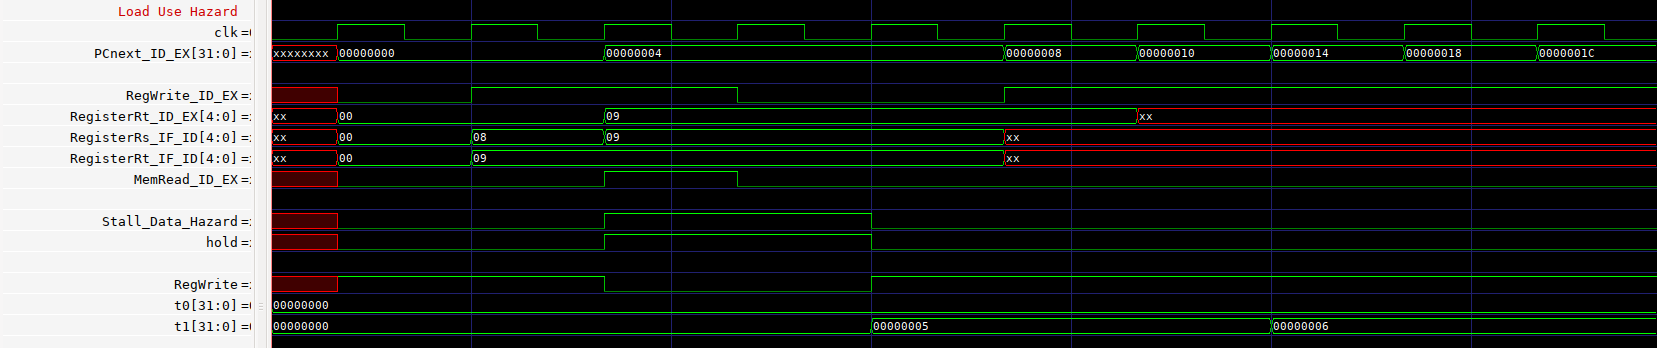
\includegraphics[width=\columnwidth]{Lab-Tex/Lab7-images/p4.png}
    \captionof{figure}{Signals for the RAW hazard in stalling}
    \label{fig:loaduse_stall}
    \medskip
\endgroup


\subsection{Hazard Detection and Forwarding}

Given the program for forwarding, the \cc{ForwardA} signal was activated twice with separate signals to forward the value. Figure \ref{fig:forwarding_raw}, shows that on the 4th cycle, the \cc{RegWrite-Ex-Mem} signal is already activated, the \cc{Rd-EX-MEM aka RFWRiteReg-EX-MEM} switches away from being zero and becomes equivalent to \cc{Rs-ID-EX}. As a result, \cc{Forward A} tells the ALU input to pick up the value from the ALU output of the previous instruction.\\

All of these values are shifted one cycle for the next stage of the pipeline, and also activate the MEM hazard because the \cc{Rs} does not change for all three instructions. As a result, \cc{Forward A} tells the ALU input to pick up the value from the ALU output of two instructions prior.\\

\begingroup
    \centering
    \medskip
    %width=\columnwidth
    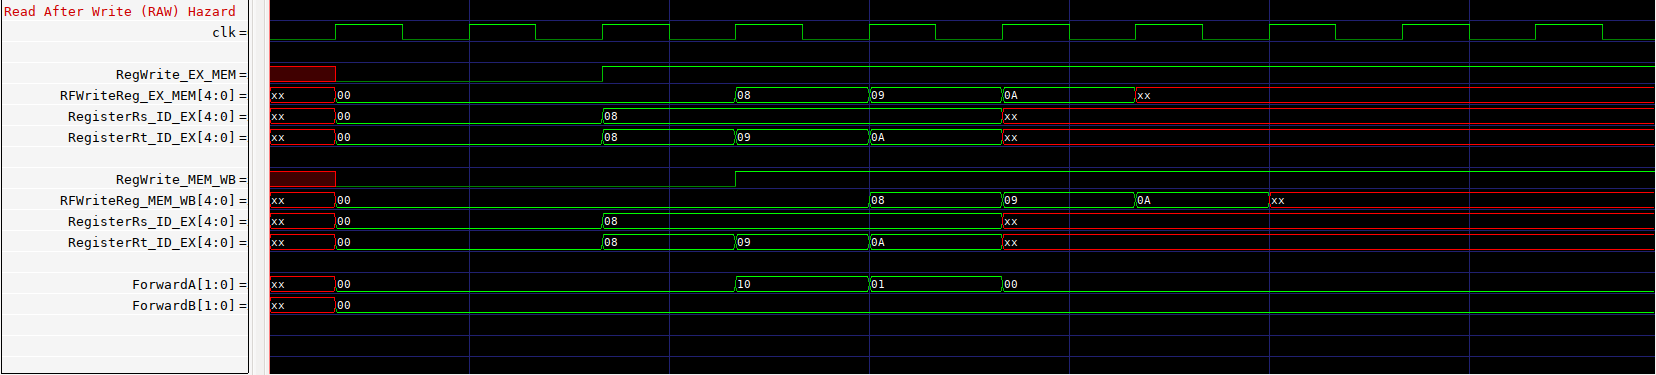
\includegraphics[width=\columnwidth]{Lab-Tex/Lab7-images/p1.png}
    \captionof{figure}{Signals for the RAW hazard in forwarding}
    \label{fig:forwarding_raw}
    \medskip
\endgroup

Figure \ref{fig:forwarding_res} shows the ALU outputs and final register values. The ALU input 1 picks up values from the registers, while ALU input 2 receives the immediate values. In the 3rd, or the EXE, stage the ALU input 2 correctly feeds the immediate value 1. We also see that the ALU input 1 correctly switches to 1, once 1 is added to register \cc{\$t0} by the 4th cycle.\\

Finally, we see that the three registers receive the proper final values, each delayed by one cycle from the previous as a result of the pipeline implementation.

\begingroup
    \centering
    \medskip
    %width=\columnwidth
    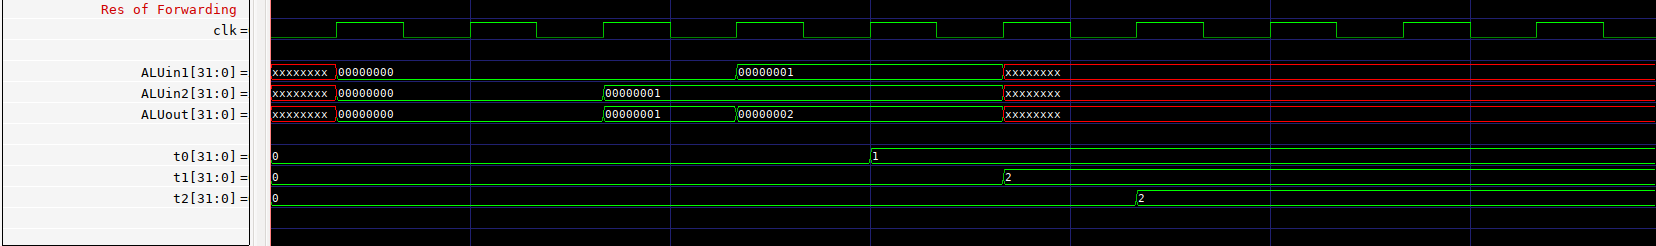
\includegraphics[width=\columnwidth]{Lab-Tex/Lab7-images/p2.png}
    \captionof{figure}{Resulting values of forwarding}
    \label{fig:forwarding_res}
    \medskip
\endgroup



\section{Conclusion}

This lab approaches a few common data hazards using stall and forwarding. Typically, the MIPs pipeline combines both approaches to solve problems like the load-use hazard. A forward and a stall is required to obtain the correct value. The stalling was a bit difficult, as it is generally not convention to stall when forwarding can do the job, as was in the case of the provided sample assembly code. Nevertheless, this exercise was able to highlight the benefit of forwarding over stalling. In the case of forwarding, no cycles were lost and the registers received the correct data. 


%%%%%%%%%%%%%%%%%%%%%%%%%%5
% BIBLIOGRAFIA 
% Estilo de bibliografia ABNT. Se não tiver instalado, mude para plain ou ieeetr

%\bibliographystyle{plain} % Inclua isso se não tiver ABNTEX instalado
% \begin{thebibliography}{refs}
% \bibitem{}
\printbibliography
% \end{thebibliography}
\end{document}